\input{def/preambule}
\begin{document}
	%%%%%%%%%%%%%%%
	%% RENEWCOMMAND
	%%%%%%%%%%%%%%%
	\renewcommand\labelitemi{\textbullet}
	\renewcommand\labelitemii{$\circ$}
	\renewcommand\labelitemiii{$\star$}
	% redefines the itemizing symbols for the itemize environment, 
	% cannot redefine the 4th lvl, 
	% cannot have more than 4 lvls,
	% in french, by default, it's all dashes...
	
	%%%%%%%%%%%%%
	%% TITLE PAGE
	%%%%%%%%%%%%%
	\input{def/titlepage}
	
	%%%%%%%%%%%%%%%%%%%
	%% TABLE OF CONTENT
	%%%%%%%%%%%%%%%%%%%
	\setcounter{page}{1} % beginning of page numeration here
	\tableofcontents
	\newpage
	
	%%%%%%%%
	%% INPUT
	%%%%%%%%
	\section{Introduction}
The purpose of this project is to design and program a mini "deep learning framework" using only pythorch's tensor operation and standard maths packages. The program should be able to compute a neural network with two inputs and two outputs with three hidden layers of 25 neurons each. The neural network should be able to provide fully connected Linear, TanH or ReLu layers and use a stochastic gradient descent with the mean square error to optimize the parameters.
	\section{Structure}
To program our neural network, we decide to separate the program in two main \mintinline{python}{class} as shown in the Figure XXXX

INSERT FIGURE

\subsection{Class neural network}

The first \mintinline{python}{class} is \mintinline{python}{NeuralNetwork}. This \mintinline{python}{class} is use to initialize the neural network and train it, it contain the following function (The complete code for \mintinline{python}{class} is in the appendix~\ref{app::NeuralNetwork}):

\begin{itemize}
	\item \mintinline{python}{def __init__(self)} : construct a empty neural network.
	\item \mintinline{python}{def sequential(self,*args)} : function to define the layer of the neural network, it need a series of constructor like Linear.
	\item \mintinline{python}{def run(self, input_data)} : Compute the result of the neural network in function of the input.
	\item \mintinline{python}{def loss(self, x, target)} : Compute the MSE loss.
	\item \mintinline{python}{def d_loss(self, x, target)} : Compute the derivative of the loss.
	\item \mintinline{python}{def test_error(self, test_input, test_label)} : compute the number of error of classification in function of a test set input and these label.
	\item \mintinline{python}{def params(self)} : Print all information of the network like layer type, number of input, number of output, weight and bias matrix for each layer.
	\item \mintinline{python}{def train_network(self, train_set, train_output, epochs, batch_size, learning_rate, print_error=False,}\\
	\mintinline{python}{test_set=None, test_label=None)} : Train the neural network with or without printing the percentage of error at each epochs in function of the boolean  \mintinline{python}{print_error}
\end{itemize}

To make the \mintinline{python}{class NeuralNetwork} work, we need a class of the layer.
 
\subsection{Layer}

The second \mintinline{python}{class} is \mintinline{python}{Linear}. This \mintinline{python}{class} ..... The \mintinline{python}{class Linear} contain the following function (The complete code for \mintinline{python}{class Linear} is in the appendix~\ref{app::Layer}) 

\begin{itemize}
	\item \mintinline{python}{def __init__(self, nb_input, nb_output)} : Create the Linear layer and initialize the weight and bias matrix.
	\item \mintinline{python}{def activation(self,x)} : Compute the activation function, in a linear layer, there is no activation function thus the function return the input.
	\item \mintinline{python}{def d_activation(self, x)} : Compute the derivative of the activation function, in a linear layer, there is no activation function thus the derivative activation return 1.
	\item \mintinline{python}{def forward_pass(self,x)} : Compute the forward pass for the layer, multiply the input by the weight and add the bias then call the activation function with the result. Return the result of the activation function. Save the input and the result of z to facilitate the computation of the backward pass
	\item \mintinline{python}{def backward_pass(self, dl_dy)} Compute the backward pass for the layer, compute the derivative of the loss in function of the weight, bias and input. Then accumulate the derivative of the weight and bias.
	\item \mintinline{python}{def update_parameters(self, learning_rate, batch_size)} : Update the parameters in function of the accumulative derivative of the weight and the bias with a learning rate.
	\item \mintinline{python}{def params(self)} : Print useful information about the current layer, his type, number of neuron input and output, shape of the weight and bias matrix and value of this matrix.
\end{itemize}

To implement the ReLu and the TanH layer, two child class was made. In this two class, the constructor, the activation and the derivative activation function are overload to have the correct function and initialization for ReLu and TanH layer. 
	\section{Initialization choice}
In this project, we use two different initialization for the weight and bias. For the TanH layer, we use the Xavier initialization, thus the weight are initialize from a random distribution with a mean of $0$ and a variance of $\dfrac{2}{size^{Layer-1}+size^{Layer}}$ and initialize the bias to $0$. For the ReLu layer, we use the He initialization which is the same initialization as Xavier initialization but with two time the variance. Those XXXXXX HELP TO 

\begin{figure}[H]
	\begin{subfigure}[h]{0.48\textwidth}
		\begin{center}
			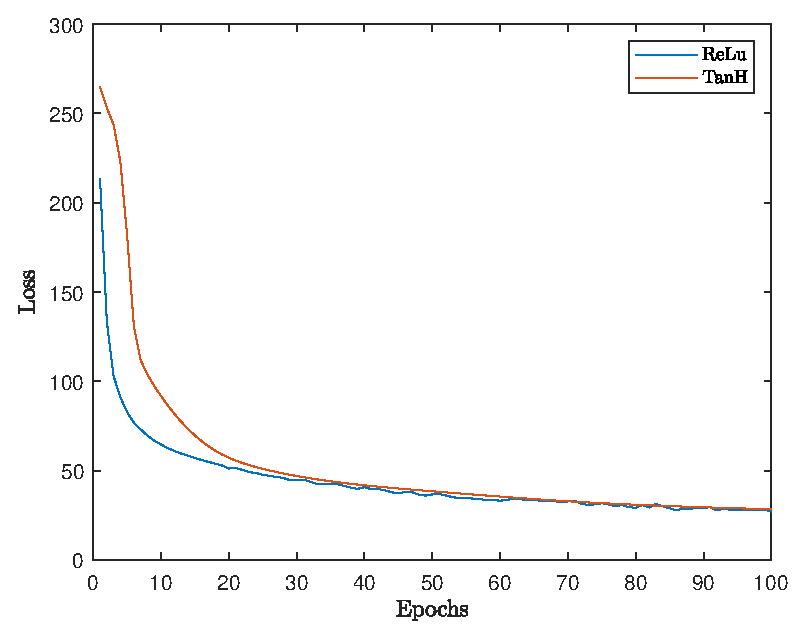
\includegraphics[width=\textwidth]{loss}
		\end{center}
	\end{subfigure}
	\begin{subfigure}[h]{0.48\textwidth}
		\begin{center}
			\includegraphics[width=\textwidth]{accuracy}
		\end{center}
	\end{subfigure}
	\caption{Average of 5 measure of loss and accuracy of the neural network $2$ input and  output and $3$ hidden layer of $25$ neuron each, with the following parameters : $100$ epochs, batch size of $1$, learning rate of $0.02$}
	\label{img::loss_accuracy}
\end{figure}

In Figure ~\ref{img::loss_accuracy}, we can see the result of two neural network with $2$ input, $2$ output and $3$ hidden layer of $25$ neuron each. The blue one is with ReLu layer and the red on is with TanH layer. We can see that the loss converge for the two type of layer. With the chosen parameters, we can see that TanH have better accuracy but is slower to converge than the ReLu layer.
	\section{Utilization}
To use the framework of this project to construct a neural network, the modules \mintinline{python}{neural_network} and \mintinline{python}{layer} have to be import.There is a example of utilization to create a neural network with $2$ input, $2$ output and $3$ hidden layer of $25$ neuron each with TanH layers (the module \mintinline{python}{neural_network} is import as \mintinline{python}{nn}) :

\begin{minted}{python}
	net = nn.NeuralNetwork()
	net.sequential(layer.TanH(2,25), layer.TanH(25,25), layer.TanH(25,25), layer.TanH(25,2))
	net.train_network(train_set, train_label, epochs=100, batch_size=1, learning_rate=0.02, print_error=True, 
						test_set=test_set, test_label=test_label)
\end{minted}

The first step is to create neural network with \mintinline{python}{NeuralNetwork()} then parameterize the neural network with the layer needed with \mintinline{python}{sequential(layer.type_layer(nb_input_layer,nb_output_layer),...)}. Then the neural network is ready to train. To train the neural network, the function \mintinline{python}{train_network} is use if the \mintinline{python}{print_error} is set to False, \mintinline{python}{test_set}and \mintinline{python}{test_label} are not needed. Thus, the train function will not compute the error for each epochs. It is important to note that they are no protection for wrong input in this function. The user have to be careful with the input (the train set and test set have to be coherent with the neural network build and batch size have to be a divider of the size of the train set).

After the training, the user freely use the neural network with the function \mintinline{python}{run(input)} and can access different log : the log of the loss with \mintinline{python}{net.graph_loss} and if \mintinline{python}{print_error=True} the log of the loss and the accuracy with \mintinline{python}{net.logs}. He can also see the parameter of the neural network by using the function \mintinline{python}{net.params()}.

\subsection{New layers}
With the chosen implementation, it is easy to add new type of layers. To add new type of layer, the user have to create a new child class form \mintinline{python}{class Linear} and overload the constructor (to initialize differently the weight and bias), the activation function and the derivative function with the new function for the layer.   
	\section{Results}
The graph below are the result of two neural network, one with TanH layer and one with ReLu layer, with the following parameters :
$2$ input, $2$ output and $3$ hidden layer of $25$ neuron each, $200$ epochs, batch size of $1$ and a learning rate of $0.02$. The training set is $1000$ random two dimensional points between $0$ and $1$ classified with a $1$ if the point is in a circle center in $[0.5,0.5]$ and radius equal to $1/\sqrt{2\pi}$ and $0$ when the point are outside. A seed is use for the random generation for the parameters to have always value to help to debug and compare the result. The complete code is in the appendix~\ref{app::code}.
\begin{figure}[H]
	\begin{subfigure}[h]{0.4\textwidth}
		\begin{center}
			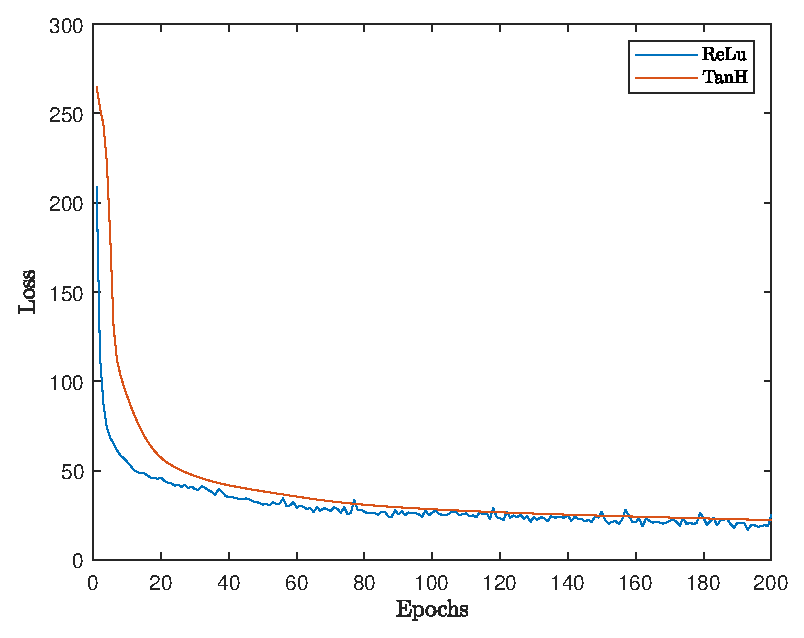
\includegraphics[width=\textwidth]{loss200}
			\caption{Loss}
		\end{center}
	\end{subfigure}
	\begin{subfigure}[h]{0.4\textwidth}
		\begin{center}
			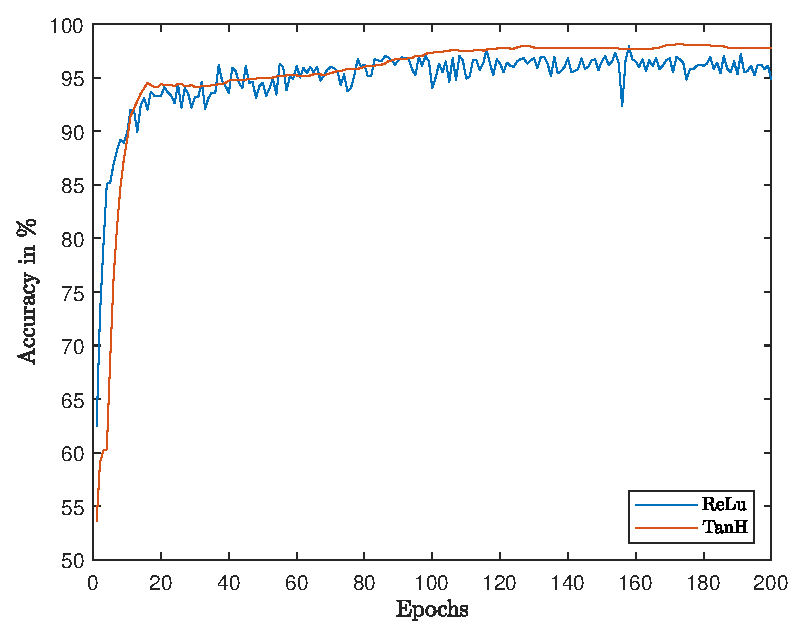
\includegraphics[width=\textwidth]{accuracy200}
			\caption{Accuracy}
		\end{center}
	\end{subfigure}
	\begin{subfigure}[h]{0.4\textwidth}
		\begin{center}
			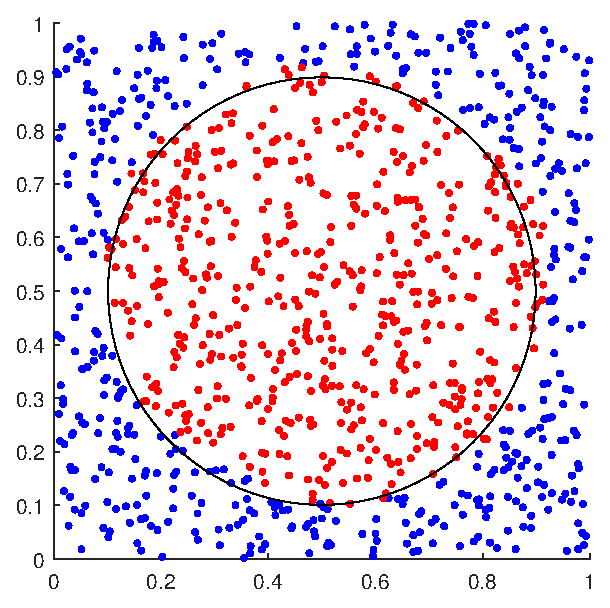
\includegraphics[width=\textwidth]{relu_out}
			\caption{Test set classified with ReLu}
		\end{center}
	\end{subfigure}
	\begin{subfigure}[h]{0.4\textwidth}
		\begin{center}
			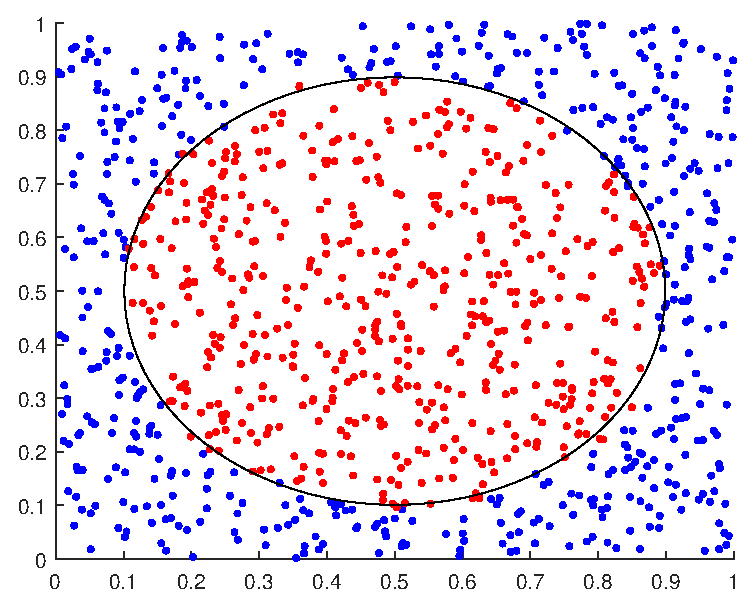
\includegraphics[width=\textwidth]{tanh_out}
			\caption{Test set classified with TanH}
		\end{center}
	\end{subfigure}
	\caption{Result of two neural network with ReLu and TanH layer with the following parameters : $2$ input, $2$ output and $3$ hidden layer of $25$ neuron each, $200$ epochs, batch size of $1$ and a learning rate of $0.02$}
	\label{img::result}
\end{figure}

The final error rate for the ReLu neural network with the test set is $5.8\%$, and $2.2\%$ with the TanH neural network.
	\section{Conclusion}
In this project, a simple neural network framework was developed with the possibility to construct neural networks  with a non-fixed numbers of fully connected Linear, ReLu or TanH layers. 
It uses the stochastic gradient descent with the mean square error as the loss function to train the network. 
It can also use the batch gradient descent, if a batch size is set.

An improvement to this framework would be to implement a more optimized gradient descent with matrix multiplication. Indeed, it would speed up things in case of batch size greater than 1, because the backward pass could take as input the loss, but in batch.
	
	%%%%%%%%%%%%%
	%% APPENDICES
	%%%%%%%%%%%%%
	\newpage
	\appendix
	\section{Code for NeuralNetwork class}
\label{app::NeuralNetwork}

%\begin{listing}[H]
%	\cprotect\caption{Package manifest.}
%	\inputminted[firstline=1,lastline=74]{xml}{../src/ros_basics_2020/package.xml}
%\end{listing}

%The \verb|urdf/macros.xacro| file contains a description of the robot's~:
%\begin{itemize}
%	\item elements' inertiae, 
%	\item sensors' dimensions
%\end{itemize}

%\inputminted[]{xml}{../urdf/macros.xacro}

%\newpage

%The \verb|urdf/materials.xacro| file contains a description of the materials used; here were only described a few colors~:

%\inputminted[]{xml}{../urdf/materials.xacro}

The \verb|neural_network.py| file contains the description of \mintinline{python}{class NeuralNetwork}~:

\inputminted[]{python}{../project2/neural_network.py}

\newpage
	\section{Code for Layer class}
\label{app::Layer}

%\begin{listing}[H]
%	\cprotect\caption{Package manifest.}
%	\inputminted[firstline=1,lastline=74]{xml}{../src/ros_basics_2020/package.xml}
%\end{listing}

%The \verb|urdf/macros.xacro| file contains a description of the robot's~:
%\begin{itemize}
%	\item elements' inertiae, 
%	\item sensors' dimensions
%\end{itemize}

%\inputminted[]{xml}{../urdf/macros.xacro}

%\newpage

%The \verb|urdf/materials.xacro| file contains a description of the materials used; here were only described a few colors~:

%\inputminted[]{xml}{../urdf/materials.xacro}

The \verb|layer.py| file contains the description of \mintinline{python}{class Linear} and the \mintinline{python}{class} which is derived from it:

\inputminted[]{python}{../project2/layer.py}

\newpage

	%%%%%%%%%%%%%%%
	%% BIBLIOGRAPHY
	%%%%%%%%%%%%%%%
	\newpage
	\section*{Bibliography} % to add a section-like unnumbered title
	\addcontentsline{toc}{section}{Bibliography} % to add said title to the toc
	\markboth{Bibliography}{Bibliography} % to modify the header
	\printbibliography[
		heading=subbibintoc,
		type=article,
		title={Articles}
	]
	
\end{document}